%%%%%%%%%%%%%%%%%%%%%%%%%%%%%%%%%%%%%%%%%%%%%%%%%%%%%%%%%%%%%%%%%%%
%
% Ce gabarit peu servir autant les philosophes que les scientifiques ; 
% et même d'autres genres, vous en faites ce que vous voulez.
% J'ai modifié et partagé ce gabarit afin d'épargner à d'autres 
% d'interminables heures à modifier des gabarits d'articles anglais. 
% 
% L'ajout d'une table des matières et une bibliographie a été ajoutée,
% rendant le gabarit plus ajusté aux besoins de plusieurs.
%
% Pour retrouvé le gabarit original, veuillez télécharger les
% documents suivants: llncs2e.zip (.cls et autres) et 
% typeinst.zip (.tex). Les documents ci-haut mentionnés ne sont pas 
% disponibles au même endroit, alors je vous invite à fouiller le web. 
%
% Pour l'instant (02-2016) ils sont disponibles tous deux ici :
%
% http://kawahara.ca/springer-lncs-latex-template/
%
% Netkompt
%
%%%%%%%%%%%%%%%%%%%%%%%%%%%%%%%%%%%%%%%%%%%%%%%%%%%%%%%%%%%%%%%%%%%


%%%%%%%%%%%%%%%%%%%%%%% file typeinst.tex %%%%%%%%%%%%%%%%%%%%%%%%%
%
% This is the LaTeX source for the instructions to authors using
% the LaTeX document class 'llncs.cls' for contributions to
% the Lecture Notes in Computer Sciences series.
% http://www.springer.com/lncs       Springer Heidelberg 2006/05/04
%
% It may be used as a template for your own input - copy it
% to a new file with a new name and use it as the basis
% for your article.
%
% NB: the document class 'llncs' has its own and detailed documentation, see
% ftp://ftp.springer.de/data/pubftp/pub/tex/latex/llncs/latex2e/llncsdoc.pdf
%
%%%%%%%%%%%%%%%%%%%%%%%%%%%%%%%%%%%%%%%%%%%%%%%%%%%%%%%%%%%%%%%%%%%

\documentclass[runningheads,a4paper]{llncs}

\usepackage[utf8]{inputenc}

\usepackage{natbib}
\bibliographystyle{apalike-fr}

\usepackage{amssymb}
\setcounter{tocdepth}{3}
\usepackage{graphicx}

\usepackage[french]{babel} % Pour adopter les règles de typographie française
\usepackage[T1]{fontenc} % Pour que les lettres accentuées soient reconnues

\usepackage{url}
\urldef{\mailsa}\path|{alfred.hofmann, ursula.barth, ingrid.haas, frank.holzwarth,|
\urldef{\mailsb}\path|anna.kramer, leonie.kunz, christine.reiss, nicole.sator,|
\urldef{\mailsc}\path|erika.siebert-cole, peter.strasser, lncs}@springer.com|    
\newcommand{\keywords}[1]{\par\addvspace\baselineskip
\noindent\keywordname\enspace\ignorespaces#1}

\begin{document}

\mainmatter 

\title{Fouille de données}

\titlerunning{Fouille de données: Data Mining}

\author{Mokeddem Sid Ahmed}

\institute{Université de Mostaganem Abdelhamid Ibn Badis}

\authorrunning{Mokeddem Sid Ahmed}

\toctitle{Résumé}
	
\tocauthor{{}}

\maketitle

\begin{abstract}
Les algorithmes de fouille de données forment la base d'un domaine très à la mode au monde de traitement automatique des données c'est la "Science de données, ou bien Data Science" , ce domaine inclut des méthodes automatiques pour l'analyse des motifs et modèles pour tout type de données, ces applications ont une grande ampleur sur différents domaines tels que le business intelligence. 

Ces notes de cours est destinées aux étudiants de Master 2 ISI. Elles permettent d'initier les étudiants au domaine de la science des données en présentant l'approche fouille de données en intégrant les concepts prérequis de l'apprentissage machine et statistique. Cependant, le document est structuré comme suivant: 
\begin{itemize}
  \item Analyse de données exploratoire
  \item Extraction des motifs fréquents (pattern mining)
  \item Clustering
  \item Classification
\end{itemize}   
Ce document montre les bases de ces approches et couvre l'analyse en big data, avec des exemples et une comparaison des différents algorithmes, ce document est un guide de fouille de données pour les étudiants et les chercheurs. 
\end{abstract}
\medskip

\begingroup
\let\clearpage\relax
\tableofcontents
\addcontentsline{toc}{section}{Introduction}
\endgroup

\medskip
\medskip

\section*{Introduction}
Ces dernières années, le domaine de science de données a connu une forte accélération avec l’apparition du phénomène BIG DATA.

Les caractéristiques des « données » ont singulièrement évolué surtout par l’évolution technologique (internet est un média incontournable, les capacités de stockages évoluent fortement, etc.), de par nos pratiques de communication (les réseaux sociaux, les forums, etc.), par la multiplication des sources et des formats des informations transmises (textes, images, vidéo avec les plates-formes d’échange, etc.). Ce phénomène désigne les  caractéristiques des données par les termes : volume, variété, vélocité.

De ce fait, de nouveaux contraintes apparaissent pour soulever l’évolution de la spécialité où l’objectif reste néanmoins toujours la valorisation des données par des techniques informatiques tels que l'apprentissage machine ou statistique: big analytics, big data analytics, business analytics, etc. Ces techniques peuvent être rassembler sous le terme générique DATA SCIENCE, avec un nouveau métier : data scientist. Par conséquent, on peut dire que la fouille de données représente le noyau du data science d’où la nécessité de comprendre les fondement de ce domaine.  \\
la fouille de données,  dans  sa  forme  et  compréhension  actuelle,  à  la  fois  comme 
champ  scientifique  et  industriel,  est  apparu  au  début  des  années  90.  Cette 
émergence n’est pas le fruit du hasard mais le résultat de la combinaison de nombreux   facteurs à la fois technologiques, économiques  et même sociopolitiques. \\

On peut voir la fouille de données comme une nécessité imposée par le besoin des 
entreprises afin de valoriser les données stockés dans leurs base de données. En effet, avec cette explosion en matière de stockage ce qui devient un enjeu pour les entreprises (la prise de conscience de l’intérêt commercial pour l’optimisation des processus de fabrication, vente, gestion, logistique, ...), beaucoup de questions s'imposent ou la plus principale est: Que doit-on faire avec des données coûteuses à collecter et à conserver?\\
La fouille de données a aujourd’hui une grande importance  économique du fait qu’elle permet d’optimiser la gestion des ressources (humaines et matérielle). Elle est utilisée par exemple :
\begin{itemize}
\item \textbf{Organisme de crédit:} pour décider d’accorder ou non un crédit en fonction du profil du demandeur de crédit, de sa demande, et des expériences passées de prêts;
\item \textbf{organisation des rayonnages dans les supermarchés} regroupant les produits qui sont généralement achetées ensemble (pour que les clients n’oublient pas bêtement d’acheter un produit parce qu'il est situé a l’autre bout du magasin). Par exemple, on extraira une règle du genre : " les clients qui achètent le produit X en fin de semaine, pendant l’été, achètent généralement également le produit Y " ;
\item \textbf{Organisation de campagne de publicité}, promotions, ... (ciblage des offres)
\item \textbf{diagnostic médical} : "les patients ayant tels et tels symptômes et demeurant dans des agglomérations de plus de 10 4 habitants développent couramment telle pathologie " ;
\item \textbf{commerce  électronique}, recommandation de produits
\item \textbf{analyser les pratiques et stratégies commerciales} et leurs impacts sur les ventes
\item \textbf{moteur de recherche sur internet}: \textit{fouille du web}
\item \textbf{extraction d’information depuis des textes} : \textit{fouille de textes}
\end{itemize}
Dans ce cours, on s’intéressera essentiellement au différentes approches liées à la fouille de données avec l’étude de quelques exemples typiques de ces algorithmes constitue le corps de ce cours, suivie de l étude de quelques applications réelles. Avant tout, nous discutons de la notion de données.
\section{Qu’est ce qu’une données ?}
Cette section a pour objet de fixer un vocabulaire et de rappeler quelques faits importants concernant les attributs des données et ce que représente la valeur d’un attribut. Mais tout d’abord quelques notations que nous retrouverons dans l’ensemble du cours. 
\subsection{Notations}
On notera $ D $ un ensemble de données, Chaque données est décrite par un ensemble de descripteurs (attributs) $ A $. chaque attribut $ a \in A $ prend sa valeur dans un certain nombre de valeurs $ V_{a} $.  Si on a $ p $ attributs $ a_{1},...,a_{p} $. Ainsi, on peut considérer l'espace des données $ E = V_{a_{1}} \times V_{a_{2}} \times ... \times V_{a_{p}}$  qui balayent toutes valeurs possible des attributs. Toute donnée appartient à cet ensemble de données $ D \subset E $. \\
Il est utile d'avoir une représentation géométrique de l'espace des données $ E $  de $ P $ dimensions ou chaque attribut correspond à un axe. 
\subsection{Types d'attributs}
Une donnée est un \emph{enregistrement (tuple)} au sens des bases de données, que l’on nomme aussi "\emph{individu}" (terminologie issue des statistiques) ou "\emph{instance}" (terminologie orientée objet en informatique) et "\emph{point}" ou "\emph{vecteur}" parce que finalement, d’un point de vue abstrait, une donnée est un point dans un espace euclidien ou un vecteur dans un espace vectoriel. Une donnée $ d $ est décrite par un ensemble d'attributs d’attributs $ A $. Un attribut $ a $ peut être de nature qualitative ou quantitative en fonction de $ V_{a} $.\\
\textbf{Attribut qualitatif}, si on peut pas faire une moyenne (une couleur, une marque de voiture, ...). Sinon \textbf{l'attribut quantitatif} : un entier, un réel, ...; il peut représenter un salaire, age, nombre d'habitants, etc., donc les opérations arithmétique habituels sont applicable ce qui est le cas des attributs qualitatifs.
\paragraph{\textbf{Remarque:}} un attribut quantitatif ne signifie pas \emph{numérique}, et réciproquement: un code postal est numérique mais pas quantitatif. 	
\subsection{Type d'attributs par nature de leur valeurs}
Si on veut un typage raffiné des attributs il faut analyser les valeurs de ces derniers. Naturellement ces valeurs sont censées représenter une certaine mesure afin de calculer une quantité dans ce monde. On voit donc apparaître des distinctions plus subtiles entre des attributs dont les valeurs sont arbitraires et incomparables \textbf{attribut nominal}, par exemple couleur, on peut pas comparer vert est blanc. On peut dire que la température aujourd'hui est 10 C et qu'hier, il faisait 18 C, on peut dire que la température était élevé hier par rapport à aujourd'hui, donc on peut comparer les valeurs, d’où un attribut, avec des valeurs arbitraires et incomparables, est un \textbf{attribut ordinal}. Les attributs  avec des valeurs non arbitraires sont considérés comme \textbf{attribut absolu} , par exemple, le nombre d'enfant. Ces différentes natures entraînent le fait que les opérations que l’on peut faire sur ces attributs ne sont pas les mêmes.
\subsection{Bruit}
Un ensemble de données $ D $ est généralement contraint à des attributs avec des valeurs inconnue ou encore moins des valeur non valide ; il faut donc gérer des données dont certains attributs ont une valeur inconnue ou invalide ; on dit que les données sont \textbf{Bruitées}.  La simple  élimination des données ayant un attribut dont la valeur est inconnue ou invalide pourrait vider complètement la base de données! alors quand on fait de la fouille de données on effectue de nombreuses opérations sur les données hors, selon la nature de l’attribut, ces
opérations sont licites ou non... Il importe donc de ne pas faire n’importe quel calcul, d’appliquer n’importe quel algorithme sans prendre garde aux attributs sur lesquels on les effectue d’où la nécessite d'une phase de \emph{prétraitement de données}. 

\section{Extraction des connaissances à partir des données}
Une  confusion  subsiste  encore  entre fouille de données et knowledge  discovery  in  data  bases (KDD) (Extraction des connaissances à partir des données (ECD)). La fouille de données est l’un des maillons du processus de traitement pour la découverte des connaissances à partir des données. Sous forme imagée, nous pourrions dire que l’ECD est un véhicule dont la fouille de données est le moteur. \\
La fouille de données représente le noyau du processus de découverte des connaissances à partir des données. Les données  peuvent  être  stockées  dans  des  entrepôts (data  warehouse),  ou sur n'importe quel support de stockage. La fouille de données ne se limite pas   au   traitement   des   données   structurées   sous   forme   de   tables; il offre des moyens pour aborder les corpus en langage naturel(fouille de texte), les images (fouille des images), le son (sound mining) ou la vidéo et dans ce cas, on parle alors plus généralement de multimedia mining.\\
L’ECD  est  un  processus  complexe  qui  se  déroule  suivant  une  série d’opérations. Des étapes de prétraitement ont lieu avant la fouille de données. 
\subsection{Étape de prétraitement}
Le  prétraitement porte sur l’accès aux données en vue de construire des datamarts, des   corpus   de   données spécifiques. Le prétraitement  concerne  la  mise  en  forme  des  données  entrées  selon  leur  type (numériques,  symboliques,  images,  textes,  sons),  ainsi  que  le  nettoyage  des  données, le traitement des données manquantes, la sélection d’attributs ou la sélection d’instances. Cette première phase est cruciale car du choix des descripteurs  et  de  la  connaissance  précise  de  la  population  va  dépendre  la mise au point des modèles de prédiction. L’information nécessaire à la construction d’un bon modèle de prévision peut être disponible dans les données  mais  un  choix  inapproprié  de  variables  ou  d’échantillon d’apprentissage peut faire échouer l’opération.



%Vous trouverez des informations pertinentes concernant ce gabarit (en anglais)
%dans le reste de ce document.
%
%The \LaTeX{} source of this instruction file for \LaTeX{} users may be
%used as a template. This is
%located in the ``authors'' subdirectory in
%\url{ftp://ftp.springer.de/pub/tex/latex/llncs/latex2e/instruct/} and
%entitled \texttt{typeinst.tex}. There is a separate package for Word 
%users. Kindly send the final and checked source
%and PDF files of your paper to the Contact Volume Editor. This is
%usually one of the organizers of the conference. You should make sure
%that the \LaTeX{} and the PDF files are identical and correct and that
%only one version of your paper is sent. It is not possible to update
%files at a later stage. Please note that we do not need the printed
%paper.
%
%\section{Première section}
%
%Vous trouverez des informations pertinentes concernant ce gabarit (en anglais)
%dans le reste de ce document.
%
%The \LaTeX{} source of this instruction file for \LaTeX{} users may be
%used as a template. This is
%located in the ``authors'' subdirectory in
%\url{ftp://ftp.springer.de/pub/tex/latex/llncs/latex2e/instruct/} and
%entitled \texttt{typeinst.tex}. There is a separate package for Word 
%users. Kindly send the final and checked source
%and PDF files of your paper to the Contact Volume Editor. This is
%usually one of the organizers of the conference. You should make sure
%that the \LaTeX{} and the PDF files are identical and correct and that
%only one version of your paper is sent. It is not possible to update
%files at a later stage. Please note that we do not need the printed
%paper.
%
%\subsubsection{Headings.}
%
%Headings should be capitalized
%(i.e., nouns, verbs, and all other words
%except articles, prepositions, and conjunctions should be set with an
%initial capital) and should,
%with the exception of the title, be aligned to the left.
%Words joined by a hyphen are subject to a special rule. If the first
%word can stand alone, the second word should be capitalized.
%
%Here are some examples of headings: ``Criteria to Disprove
%Context-Freeness of Collage Language", ``On Correcting the Intrusion of
%Tracing Non-deterministic Programs by Software", ``A User-Friendly and
%Extendable Data Distribution System", ``Multi-flip Networks:
%Parallelizing GenSAT", ``Self-determinations of Man".
%
%\subsubsection{Lemmas, Propositions, and Theorems.}
%
%The numbers accorded to lemmas, propositions, and theorems, etc. should
%appear in consecutive order, starting with Lemma 1, and not, for
%example, with Lemma 11.
%
%\subsection{Figures}
%
%For \LaTeX\ users, we recommend using the \emph{graphics} or \emph{graphicx}
%package and the \verb+\includegraphics+ command.
%
%Please check that the lines in line drawings are not
%interrupted and are of a constant width. Grids and details within the
%figures must be clearly legible and may not be written one on top of
%the other. Line drawings should have a resolution of at least 800 dpi
%(preferably 1200 dpi). The lettering in figures should have a height of
%2~mm (10-point type). Figures should be numbered and should have a
%caption which should always be positioned \emph{under} the figures, in
%contrast to the caption belonging to a table, which should always appear
%\emph{above} the table; this is simply achieved as matter of sequence in
%your source.
%
%Please center the figures or your tabular material by using the \verb+\centering+
%declaration. Short captions are centered by default between the margins
%and typeset in 9-point type (Fig.~\ref{fig:example} shows an example).
%The distance between text and figure is preset to be about 8~mm, the
%distance between figure and caption about 6~mm.
%
%To ensure that the reproduction of your illustrations is of a reasonable
%quality, we advise against the use of shading. The contrast should be as
%pronounced as possible.
%
%If screenshots are necessary, please make sure that you are happy with
%the print quality before you send the files.
%\begin{figure}
%\centering
%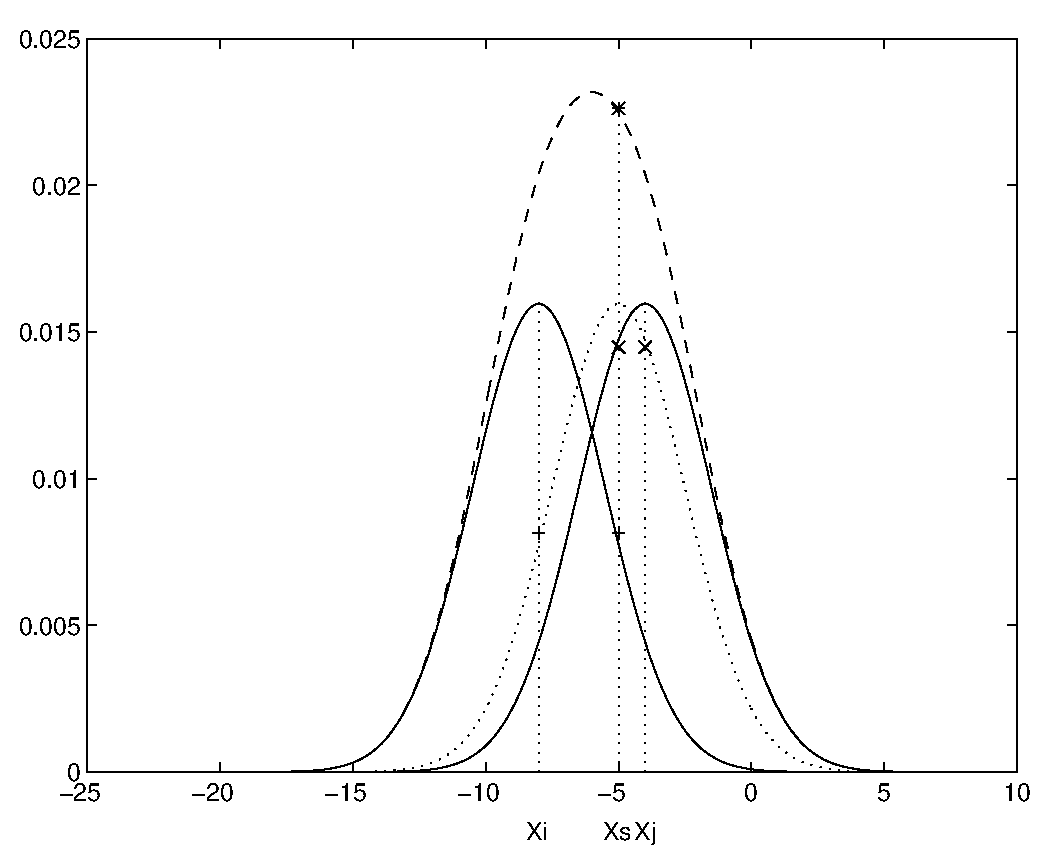
\includegraphics[height=6.2cm]{eijkel2}
%\caption{One kernel at $x_s$ (\emph{dotted kernel}) or two kernels at
%$x_i$ and $x_j$ (\textit{left and right}) lead to the same summed estimate
%at $x_s$. This shows a figure consisting of different types of
%lines. Elements of the figure described in the caption should be set in
%italics, in parentheses, as shown in this sample caption.}
%\label{fig:example}
%\end{figure}
%
%Please define figures (and tables) as floating objects. Please avoid
%using optional location parameters like ``\verb+[h]+" for ``here".
%
%\paragraph{Remark 1.}
%
%In the printed volumes, illustrations are generally black and white
%(halftones), and only in exceptional cases, and if the author is
%prepared to cover the extra cost for color reproduction, are colored
%pictures accepted. Colored pictures are welcome in the electronic
%version free of charge. If you send colored figures that are to be
%printed in black and white, please make sure that they really are
%legible in black and white. Some colors as well as the contrast of
%converted colors show up very poorly when printed in black and white.
%
%\subsection{Formulas}
%
%Displayed equations or formulas are centered and set on a separate
%line (with an extra line or halfline space above and below). Displayed
%expressions should be numbered for reference. The numbers should be
%consecutive within each section or within the contribution,
%with numbers enclosed in parentheses and set on the right margin --
%which is the default if you use the \emph{equation} environment, e.g.,
%\begin{equation}
%  \psi (u) = \int_{o}^{T} \left[\frac{1}{2}
%  \left(\Lambda_{o}^{-1} u,u\right) + N^{\ast} (-u)\right] dt \;  .
%\end{equation}
%
%Equations should be punctuated in the same way as ordinary
%text but with a small space before the end punctuation mark.
%
%\subsection{Footnotes}
%
%The superscript numeral used to refer to a footnote appears in the text
%either directly after the word to be discussed or -- in relation to a
%phrase or a sentence -- following the punctuation sign (comma,
%semicolon, or period). Footnotes should appear at the bottom of
%the
%normal text area, with a line of about 2~cm set
%immediately above them.\footnote{The footnote numeral is set flush left
%and the text follows with the usual word spacing.}
%
%\subsection{Program Code}
%
%Program listings or program commands in the text are normally set in
%typewriter font, e.g., CMTT10 or Courier.
%
%\section{Deuxième section}
%
%\subsection{ainsi de suite...}
%
%\medskip
%
%\noindent
%{\it Example of a Computer Program}
%\begin{verbatim}
%program Inflation (Output)
%  {Assuming annual inflation rates of 7%, 8%, and 10%,...
%   years};
%   const
%     MaxYears = 10;
%   var
%     Year: 0..MaxYears;
%     Factor1, Factor2, Factor3: Real;
%   begin
%     Year := 0;
%     Factor1 := 1.0; Factor2 := 1.0; Factor3 := 1.0;
%     WriteLn('Year  7% 8% 10%'); WriteLn;
%     repeat
%       Year := Year + 1;
%       Factor1 := Factor1 * 1.07;
%       Factor2 := Factor2 * 1.08;
%       Factor3 := Factor3 * 1.10;
%       WriteLn(Year:5,Factor1:7:3,Factor2:7:3,Factor3:7:3)
%     until Year = MaxYears
%end.
%\end{verbatim}
%%
%\noindent
%{\small (Example from Jensen K., Wirth N. (1991) Pascal user manual and
%report. Springer, New York)}

\bibliography{references}
\nocite{*} 

\end{document}
